\documentclass[fontsize=12pt,		% Font size
			   toc=listof,			% List of... into table of contents % listofnumbered
			   paper=A4,			% A4 paper
			   headinclude=true,	% Include header into type area calculation
			   footinclude=false,	% Don't include footer into type area calculation
			   headsepline=true,	% Separating line between header and text
			   footsepline=false,	% Separating line between footer and text
			   DIV=calc,			% Auomatically calculate DIV
			   %BCOR=15mm,			% Binding correction
			   %twosided=true,
			   %open=right
			  ]{scrartcl}

\usepackage[english,ngerman]{babel}
\addto\extrasngerman{%
 \def\subsubsectionautorefname{Unterabschnitt}%
}
\usepackage[utf8]{inputenc}
\usepackage[babel,german=guillemets]{csquotes}
\usepackage[T1]{fontenc}
\usepackage[onehalfspacing]{setspace}

\usepackage{lmodern}
\usepackage{microtype}

\usepackage{textcomp}				% Avoids conflicts between siunitx and microtype
\usepackage{siunitx}				% Allow for german decimals, e.g. 1,344 instead of 1.344 + other stuff

\usepackage{graphicx}
\usepackage{listings}
\usepackage{color}
\usepackage{hyperref}
\usepackage{pdfpages}

\usepackage{relsize}
\usepackage{subfigure}

% Package and options for nice inspirational quotes - takes one argument - the author of the quote.
\makeatletter
%\renewcommand{\@chapapp}{}% Not necessary...
\newenvironment{chapquote}[2][2em]
  {\setlength{\@tempdima}{#1}%
   \def\chapquote@author{#2}%
   \parshape 1 \@tempdima \dimexpr\textwidth-2\@tempdima\relax%
   \itshape}
  {\par\normalfont\hfill--\ \chapquote@author\hspace*{\@tempdima}\par\bigskip}
\makeatother


% Autorenangabe
\newcommand\mychapter[2]{\chapter{#2}\vspace{-1.5em}\hspace{2.1em}\emph{#1}\vspace{1.5em}}
\newcommand\mysection[2]{\section{#2}\vspace{-0.9em}\hspace{2.1em}\emph{#1}\vspace{1.5em}}
\newcommand\mysubsection[2]{\subsection{#2}\vspace{-0.5em}\hspace{3.2em}\emph{#1}\vspace{1.3em}}
\newcommand\mysubsubsection[2]{\subsubsection{#2}\vspace{-0.5em}\hspace{3.2em}\emph{#1}\vspace{1.3em}}

% C#
\newcommand{\CS}{C\nolinebreak[4]\hspace{-.05em}\raisebox{.4ex}{\relsize{-2}{\textbf{\#}}}}

% PDF Metadaten

\pdfinfo{
 /Title (Untersuchung des Phänomens Crowdfunding)
 /Author (Sarah Häfele)
}


\begin{document}

%%%%%%%%%%%%%%%%%%%%%%%%%%%%%%%%%%%%%%%%%
% University Assignment Title Page 
% LaTeX Template
% Version 1.0 (27/12/12)
%
% This template has been downloaded from:
% http://www.LaTeXTemplates.com
%
% Original author:
% WikiBooks (http://en.wikibooks.org/wiki/LaTeX/Title_Creation)
%
% License:
% CC BY-NC-SA 3.0 (http://creativecommons.org/licenses/by-nc-sa/3.0/)
% 
% Instructions for using this template:
% This title page is capable of being compiled as is. This is not useful for 
% including it in another document. To do this, you have two options: 
%
% 1) Copy/paste everything between \begin{document} and \end{document} 
% starting at \begin{titlepage} and paste this into another LaTeX file where you 
% want your title page.
% OR
% 2) Remove everything outside the \begin{titlepage} and \end{titlepage} and 
% move this file to the same directory as the LaTeX file you wish to add it to. 
% Then add \input{./title_page_1.tex} to your LaTeX file where you want your
% title page.
%
%%%%%%%%%%%%%%%%%%%%%%%%%%%%%%%%%%%%%%%%%

%----------------------------------------------------------------------------------------
%	PACKAGES AND OTHER DOCUMENT CONFIGURATIONS
%----------------------------------------------------------------------------------------

%\documentclass[12pt]{article}

%\begin{document}

\begin{titlepage}

\newcommand{\HRule}{\rule{\linewidth}{0.5mm}} % Defines a new command for the horizontal lines, change thickness here

\center % Center everything on the page
 
%----------------------------------------------------------------------------------------
%	HEADING SECTIONS
%----------------------------------------------------------------------------------------

\Large Hochschule Furtwangen - Fakultät Digitale Medien\\[0.5cm] % Name of your university/college
{\Large \bfseries Game Development}\\[0.5cm] % Major heading such as course name
\large Sommersemester 2015\\[0.5cm] % Minor heading such as course title

%----------------------------------------------------------------------------------------
%	TITLE SECTION
%----------------------------------------------------------------------------------------

\HRule \\[0.2cm]
{ \huge \bfseries Game Design Dokument}\\ \vfill 
{ \normalsize für das Spiel}\\ \vfill 
{\huge \bfseries inCubed }\\[0cm] % Title of your document
\HRule \\[0.7cm]
 
%----------------------------------------------------------------------------------------
%	AUTHOR SECTION
%----------------------------------------------------------------------------------------

\begin{minipage}{0.55\textwidth}
\begin{flushleft} \large
\begin{singlespace}
%\emph{Authoren:}\\
Sandra Beuck\\
Lydia Friedrich\\
Fabian Gärtner\\
Sarah Häfele\\
Alexander Scheurer\\

\end{singlespace}
\end{flushleft}
\end{minipage}
~
\begin{minipage}{0.4\textwidth}
\begin{flushright} \large
%\emph{Supervisor:} \\
Prof. Dell´Oro-Friedl\\
Prof. Müller\ % Supervisor's Name
\end{flushright}
\end{minipage}\\[2cm]

% If you don't want a supervisor, uncomment the two lines below and remove the section above
%\Large \emph{Author:}\\
%John \textsc{Smith}\\[3cm] % Your name

%----------------------------------------------------------------------------------------
%	DATE SECTION
%----------------------------------------------------------------------------------------

{\large \today , Version: 1.00}\\[3cm] % Date, change the \today to a set date if you want to be precise

%----------------------------------------------------------------------------------------
%	LOGO SECTION
%----------------------------------------------------------------------------------------

%
\includegraphics{Logo}\\[1cm] % Include a department/university logo - this will require the graphicx package
 
%----------------------------------------------------------------------------------------

\vfill % Fill the rest of the page with whitespace

\end{titlepage}
\cleardoublepage
%\end{document}

%\include{Abstract}

\tableofcontents

%Bitte im folgenden \input{} nutzen!

\clearpage
\section{Einleitung}
Im Rahmen der Prüfungleistung für das Modul Game Development soll im interdisziplinären Team aus den Masterstudiengängen Design Interaktiver Medien und Medieninformatik innerhalb von vier Arbeitstagen ein Spiel entwickelt werden. Das Spiel soll auf einem mobilen Endgerät mit Hilfe der VR/AR-Brille ZEISS VR-ONE gespielt werden können. Das Thema ist: 

\enquote{Positionierung und Bewegung gleichberechtigt in allen Dimensionen im Raum}.

Das vorliegende Dokument stellt die Dokumentation der Designentscheidungen und Rahmenbedingungen dar.

(\emph{Anmerkung:} Folgend soll bei jeder männlichen Form die weibliche impliziert sein.)


\clearpage
%\section{Design History}
%\input{Sequenzdiagramm}

\clearpage
\section{Ideenfindung}
\mysubsection{Sarah Häfele}{Erste Ideen}

Nach der ersten Phase des ungeordneten Brainstormings zeichnen sich zwei verschiedene Spielideen ab, die zum Thema passen würden:
\begin{itemize}
\item Kleine schwebende Welten oder Inseln, die man durch Manipulation der Gravitation erreichen kann.
\item Die Spielwelt als Würfel, dessen Seiten voneinander abhängig sind und die sich alle verändern, wenn man eine Seite manipuliert.
\end{itemize}

Ausgewählt wird die Würfelwelt. Der Überlegung liegt ein Geschicklichkeitsspiel namens \enquote{Oskar's Cube} (siehe  Abbildung \ref{fig:Oskar}) zu Grunde. Die sechs Flächen des Würfels sind Labyrinthe, durch die man mit Stäben den Weg finden muss. Die Stäbe sind in der Mitte des Würfels miteinander verbunden, was sie zu voneinander abhängige Achsen werden lässt.

\begin{figure}[ht]%[htbp]
	\centering
		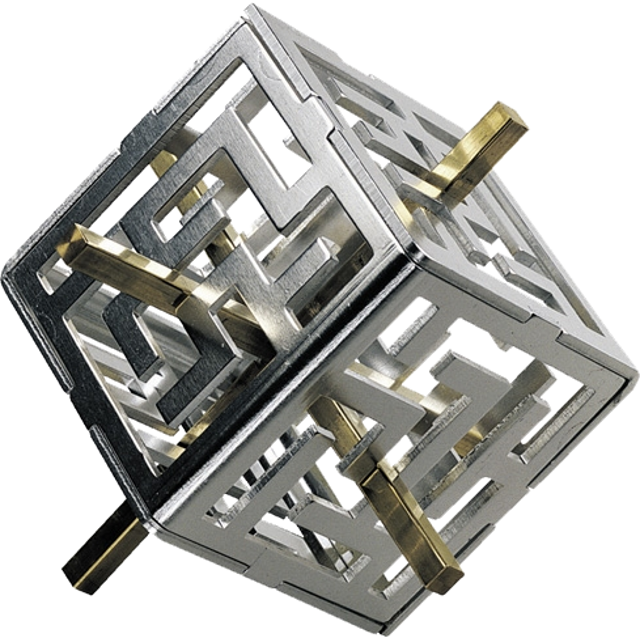
\includegraphics[width=0.6\textwidth]{images/oscar}
	\caption{Oskar's Cube (Quelle: http://www.puzzlemaster.ca)}
	\label{fig:Oskar}
\end{figure}

Die Idee eines Würfels, der die Spielwelt beschränkt, kann aus verschiedenen Gründen attraktiv sein. Die ZEISS VR-ONE ist nicht nur eine VR-Brille, sondern hat auch eine transparente Front, durch die die Handykamera aufnehmen kann. Dieses Feature soll im Konzept mit aufgenommen werden, denn es stellt einen der Unique Sellingpoints der Brille dar. Die Würfelwelt kann als Repräsentation eines Markerwürfels gesehen werden. Der Spieler hat sozusagen die Welt in der Hand und kann sie durch drehen des Markers und interner Markererkennung drehen und navigieren. 
Ein Würfel stellt durch seine sechs Seiten zudem spannende Anforderungen aber auch Freiheiten an das Art-Team bezüglich der Weltgestaltung: wie können diese interessant gestaltet werden, um den Spieler zu fesseln?
Trotzdem bietet der Würfel eine abgeschlossene Welt, was ideal für einen zeitlich stark begrenzten Game Jam ist. Die klaren Seiten bieten Orientierung für den Spieler, der durch die VR-Brille schnell diese verlieren könnte.   
  

\mysubsection{Sarah Häfele}{Erste Entscheidungen}

Die Basis ist ein großer Würfel als Spielwelt. 

Die Innenseiten des Würfels stellen Welten dar, die sich gegenüber stehen. Sie sollen durch verschiedene Rätsel, die unter anderem mit der Gravitation spielen, miteinander verbunden sein. 

Durch einen Markerwürfel soll der Spieler von außen in die Welt eingreifen und sie drehen können. Somit wird der Augmented Reality Aspekt der Brille genutzt. 

Das Ziel des Spiels könnte es sein, eine bestimmte Position zu erreichen (zum Beispiel durch ein Labyrinth den Weg finden, wie es bei Oskar's Cube der Fall ist) oder bestimmte Gegenstände einzusammeln.
   
Labyrinthe sind für ein Computerspiel, welches länger Spaß machen soll, vielleicht zu unspektakulär. Die Variante des Einsammelns kann durch verschiedene Rätsel interessant gemacht werden. Die Abhängigkeit der Seiten voneinander soll dabei jedoch trotzdem erhalten bleiben.

Eine weitere Frage wirft das Leveldesign der Welten auf: soll jede Setenfläche des Würfels eine eigene Welt darstellen, oder soll es ein Thema für den gesamten Würfel geben. Die verschiedenen Themen können mit Rätseln verknüpft werden, weswegen die Entscheidung auf ein Thema je Seitenfläche fällt.

Die Position des Spielers ist ein weiterer wichtiger Punkt, der noch vor der groben Planung entschieden werden muss. Da das Spiel im Würfel stattfinden soll, könnte der Spieler sich entweder auf den jeweiligen Flächen bewegen, in der Mitte fest verankert sein oder sich komplett frei bewegen. Da das Thema eine gleichberechtigte Bewegung und Position erfordert, wird eine Kombination aus den oben genannten Optionen gewählt. Die Ausgangsbasis des Spielers befindet sich in der Mitte des Würfels, so dass er alle Landschaften überblicken kann. Er kann jedoch auch auf die Seiten gehen und dort die Welten erkunden.

\clearpage
\section{Game Overview}
\mysubsection{Sarah Häfele}{Grobes Game Konzept}

Die sechs Innenseiten eines großen Würfels stellen Spielwelten dar. Die Objekt-Models sind im Lowpoly-Style gehalten, da sie so schnell modelliert werden können (Zeit ist im Game Jam ein wichtiger Faktor), das Mobile Device diese gut darstellen kann und zudem das eckige Würfelthema so wieder aufgegriffen wird.

Der Spieler befindet sich im Zentrum des Inneren eines Würfels und sieht die Welten im First-Person-View. Jede Innenseite besitzt eine unterschiedliche Welt, wobei jede Welt im Bezug auf ihre gegenüberliegende steht und mit ihrem Paar zwei gegensätzliche Themen darstellen.    

Die Themen sind:
\begin{itemize}
\item Feuer vs. Eis
\item Wald vs. Wüste
\item Wiese vs. Gebirge
\end{itemize}

Pro Paar müssen Aufgaben durch eine Abfolge verschiedener Aktionen in beider sich gegenüberstehender Welten gelöst werden. Eventuell können verschiedene Items als Hilfe benutzt werden. Hauptziel ist es, die Teile eines kleinen Würfels wiederzufinden.

Der Spieler hält einen Markerwürfel in der Hand, der mit verschiedenen Farbflächen und Mustern markiert ist. Mit diesem kann er durch Markererkennung die virtuelle Welt drehen. Damit wird auch in der \enquote{realen} Welt wieder das Würfelthema aufgegriffen.

Der Spieler bewegt sich rein durch seinen Blick durch die Welt. Er startert immer in der Mitte des Würfels. Jede Seite hat einen Viewpoint, auf den der Spieler, wenn er ihn länger anschaut, zugleitet. Damit kann der Spieler in die Welt eintauchen und die Seiten erkunden. Wieder zurück in der Mitte kann der Spieler sich Orientierung verschaffen und die Auswirkungen seiner Aktionen überblicken.

Das Spiel heißt \enquote{inCubed}, da das englische Wort für \enquote{Kubik} oder \enquote{hoch drei} \enquote{cubed} ist und der Spieler sich in einem dreidimensionalen Würfel befindet.

Das Game Jam Thema wird durch die gleichberechtigten Seiten aufgegriffen: wenn man auf einer Seite etwas verändert, ändert sich auch etwas auf der anderen. Durch das Umschalten der Gravitation, kann man sich frei in allen Dimensionen bewegen. In einem fertigen Spiel sollten alle Seiten voneinander gleichberechtigt abhängig voneinander sein. Für den Prototypen sollen nur die sich gegenüberliegenden Wände voneinander abhängen.    
\mysubsection{Sarah Häfele}{Feature Set}

InCubed wird auf einem mobilen Gerät mit der ZEISS-VR ONE gespielt, was besondere Features ermöglicht. Das Spiel ist dadurch nicht nur mobil, sondern wird zu einer VR- und AR-Anwendung:

Die stereoskopischen Linsen der Brille geben dem Nutzer einen Tiefeneindruck in die Welt. Durch das Headtracking werden die Kopfbewegungen des Spielers in die Spielwelt übertragen. So wird das Eintauchen in die Geschichte unterstützt.

Die Brille hat im Gegensatz zu anderen VR-Headsets zusätzlich ein transparentes Sichtfeld, welches in der Anwendung ebenfalls zum Einsatz kommt. Der Spieler steuert die Welt durch einen Markerwürfel, den er physikalisch in der Hand hält. 

Dieses Zusammenspiel zwischen Realität und Virtualität wird noch durch die Geschichte aufgegriffen.

Zudem kommt der Spieler durch den Marker und durch das Headtracking komplett ohne weitere Eingabegeräte aus. Er bewegt sich durch seine Blickrichtung in der Welt fort.
\mysubsection{Sandra Beuck}{Genre und Spielkategorie}

Das Spiel ist durch seine Aufgaben zunächst ein Rätsel- / bzw. Puzzlespiel. Da der Spieler jedoch zudem Objekte und Orte finden muss und sich auch nur durch seinen Blick fortbewegt, ist das Spiel auch ein Wimmelbild und hat Adventure-Charakter.

Das Spiel lässt sich weiterhin in die, von Roger Caillois entwickelten, Kategorien Ilinx (Strudel/ Rausch) sowie Agon (Wettkampf) einordnen. 

Ilinx: Der Rausch besteht bei diesem Spiel in dem Drang etwas Neues zu erkunden sowie Abenteuer innerhalb der Spielwelt zu erleben.

Agon = Der Kampfgeist des Spielers wird durch das Lösen von Rätseln geweckt. Diese stellen dabei weitere Herausforderungen für den Spieler dar.

Eine weitere Kategorie stellt Ludus dar, denn das Spiel ist stark Regelgebunden. Ebenso muss der Spieler beim Bearbeiten der Aufgaben strategisch vorgehen um diese zu lösen und das Spiel am Ende zu gewinnen. Das Spiel kann teilweise auch der Kategorie Paida zugeordnet werden, denn der Spieler muss die Welten genau erkunden, um die Aufgaben an sich und dessen Lösungen zu finden.
\mysubsection{Lydia Friedrich}{Zielgruppe}

Zur Zielgruppe des Spiels “InCubed” zählen Menschen ganz unterschiedlicher Charaktere. So können sich einerseits Menschen mit einer hohen Affinitiät im Bereich Technik und andererseits Casual Gamers für das Spiel interessieren. Auf Grund des Speildesigns, im Low Poly Stil, ist das Spiel ebenfalls für Kinder und Jugendliche geeignet. Augenmerk liegt jedoch eher auf Menschen, welche ein großes Interesse an Games mit neu entwickelten Techniken aufweisen und auch bereit sind für diese Produkte mehr Geld auszugeben als für alltägliche Games. Notwendig für eine korrekte Spielwiedergabe ist eine gute Hardware auf einem mobilen Endgerät sowie die VR-Brille von der Firma Zeiss, welche in der Anschaffung recht teuer sein können. Der Kauf einer VR-Brille kann jedoch für viele Casual Gamer ohne ein gewisses Maß an bereitgestellten Content unattraktiv sein. Die Tendenz von Spielumgebungen im mobilen Bereich ist jedoch steigend.

Da die Dialoge im Spiel momentan nur in Deutsch zur Verfügung stehen, ist das Spiel für den deutschen Markt und darüber hinaus für Menschen, welche der Deutschen Sprache mächtig sind, geeignet. Auch auf Grund des Rätselcharakters im Spiel, ist es für viele Personen im deutschsprachigen Raum interessant. Laut einer Studie aus dem Jahr 2014 - 2015, ist das Lösen von Rätseln auf der Beliebtheitsskala der Deutschen auf Platz drei (\footnote{\textit{Quelle:} \url{http://de.statista.com/statistik/daten/studie/171168/umfrage/haeufig-betriebene-freizeitaktivitaeten/}})

\mysubsection{Sarah Häfele}{Spielfluss}

Am Anfang des Spiels wird der Spieler durch einen Teleporter von der Realität auf die virtuelle Insel transportiert, die es zu Retten gilt. Der Spieler startet in Mitten des Würfels und kann sich dort in Ruhe umschauen. Durch das Anschauen von Viewpoints kann der Spieler alle Welten besuchen. Auf jeder Welt gilt es Rätsel zu lösen, die ebenfalls mit dem Blick ausgelöst werden. Werden alle Rätsel zweier gegenüberliegender Welten gelöst, erhält der Spieler ein Teil des zerbrochenen Remote Cubes - die Fernbedienung, die die Insel am Ende wieder aufklappen lässt.
Ziel des Spiels ist es, alle Welten zu besuchen, alle Rätsel zu lösen und die (im Prototyp) drei Teile der Fernbedienung zu sammeln. 
Der Spieler kann nicht verlieren. Am Ende sieht der Spieler, wie die Insel durch ihn gerettet wird und er kommt wieder zurück in die Realität.

Der Spielfluss kann beliebig ausgedehnt werden, indem neue Rätsel hinzukommen. Angedacht ist, dass alle Welten voneinander abhängig sind. Dies wird im Prototyp nur exemplarisch durch jeweils die gegenüberliegenden Welten umgesetzt.

%\Look und Atmosphäre

\clearpage
\section{Gameplay}
\subsection{Game Progression}

\subsection{Mission und Spielerführung}

\subsection{Intro und Outro}
\mysubsubsection{Fabian Gärtner}{Technik}

BILDER ZU INTRO/OUTRO

Das Spiel soll von Anfang an den Spieler zur Hauptrolle machen, weshalb das Intro und Outro so gestaltet wurde, dass es dem Spieler deutlich vermittelt, dass er persönlich vom verrücken Wissenschaftler zu Hilfe gerufen wurde. Wenn der Spieler das Spiel startet und die Brille aufsetzt, sieht er daher zunächst - nach einem Ladebildschirm - über die Kamera des Smartphones die Realwelt vor sich. Ein Text auf dem Bildschirm erklärt anschließend, dass der Spieler nun seinen magischen Würfel wie gezeigt (mit dem Stern zur Kamera) in das Bild halten soll. Tut er dies für fünf Sekunden, beginnt eine Sequenz, die den Spieler aus der Realwelt in die Spielwelt teleportiert. Auch hier wird das Spiel der Themenvorgabe gerecht, da der Spieler eine Reise von der Realität in die virtuelle Welt, also zwischen verschiedenen Dimensionen, miterlebt. Vermittelt wird dem Spieler diese Reise visuell durch das Einfrieren, Drehen, Verschwimmen und Überlichten des Kamerabildes und das anschließende Einblenden einer drehenden Spirale. Gleichzeitig wird diese Sequenz als eine Einleitung in das Spiel genutzt, indem dem Spieler die Vorgeschichte visuell über sechs hereinfliegende Comics und auditiv durch einen Erzähler vermittelt wird. Nach diesem Intro landet der Spieler innerhalb des dunklen Würfels und kann mit der Erkundung der Welt beginnen.

Das Outro beginnt, sobald der Spieler alle Rätsel gelöst hat. Da nun der Remote Cube wieder zusammengesetzt und funktionsfähig ist, beginnt sich die Welt um den Spieler herum aufzuklappen und eine Insel zu bilden. Zum ersten Mal sieht der Spieler dadurch den Bereich außerhalb des Würfels, der vor allem durch seine Low-Poly-Skybox auffällt, die sowohl den Himmel als auch das Wasser um die aufgeklappte Würfel-Welt herum darstellt und ebenfalls eine würfelartige Form hat. Des Weiteren erkennt der Spieler nun, da er von oben auf den aufgeklappten Würfel schaut, dass diese Welt tatsächlich auch als Insel die Form eines Würfels hat und kann daher nachvollziehen, warum der verrückte Wissenschaflter derartige Vermutungen hatte. Nach zehn Sekunden beginnt dann das Bild zu überlichten und die Rückreise für den Spieler steht an. Während der drehenden Spirale dankt der verrücke Wissenschaftler dem Spieler erneut auditiv während wiederum Comics sowohl die Story komplettieren, als auch den Abspann für das Spiel bilden. Anschließend überblendet das Spiel noch einmal und der Spieler sieht wieder das reale Kamerabild - er ist also zurück in der Realität.


\mysubsubsection{Sandra Beuck}{Art}

Hallo

\clearpage
\section{Mechaniken}
\mysubsection{Lydia Friedrich}{Allgemeine Struktur}

%\input{Physik}
\subsection{Steuerung}
\mysubsubsection{Fabian Gärtner}{Physikalische Steuerung}

Da die Steuerung für den Spieler so einfach wie möglich gehalten werden soll, sodass auch Personen, die bisher nicht mit Videospielen und der entsprechenden Peripherie (also bspw. Controller) vertraut sind, inCubed spielen können, ist jegliche Interaktion mit dem Spiel durch Blickkontakt mit Interaktionspunkten möglich. Es ist allerdings, sei es aus Platzmangel oder aus gesundheitlichen Gründen, nicht immer möglich, sich vollständig nach hinten, oben oder unten umzusehen, was die Erkundung der Welt einschränken und damit das Lösen der Rätsel erschweren würde. Die Verwendung eines handelsüblichen Controllers zur Bewegung der Spielwelt wäre hier aber nicht sinnvoll, da dieser mit seiner Vielzahl an Tasten vor allem von ungeübten Spielern eher unintuitiv zu bedienen wäre, vor allem da durch Verwendung der VR-Brille der Controller nicht sichtbar ist. Daher steht für inCubed ein deutlich intuitiverer und unkonventioneller Controller in Form eines Würfels zur Verfügung, der sich sowohl in die Rahmenhandlung einfügt, als auch dem Spieler auf einfache Art und Weise ermöglicht, sich in der Welt umzusehen. Dazu muss er während des Spiels lediglich diesen Würfel vor die Kamera des Smartphones, das sich zwar in der VR-Brille befindet, aber durch das Sichtfenster in der VR-One die Umgebung filmen kann, halten und bei Bedarf so drehen, dass eine der sechs Würfelseiten zur Kamera zeigt. Dies führt gleichzeitig dazu, dass sich die Spielwelt entsprechend um jeweils 90° dreht und so auch andere Teile der Welt erkundet werden können, ohne dass sich der Spieler selbst umdrehen muss.

Das Design dieses Würfels, auf dessen sechs Seiten sich sechs unterschiedliche Formen (Dreieck, Stern, Rechteck, Kreis, Pentagon und Heptagon) befinden, wurde so gewählt, dass zum einen die Bewegung des Würfels durch die Kamera des Smartphones möglichst effizient und zuverlässig erkannt werden kann (mehr zum technischen Hintergrund in Kapitel X) und zum anderen so, dass er optimal zur Thematik von inCubed passt. Die Geschichte in inCubed erklärt, dass es sich bei diesem Würfel um den Hilferuf des verrückten Wissenschaftlers handelt. Da der Wissenschaftler von geometrischen Formen besessen scheint, hat er nicht nur den "Remote Cube" sondern auch diese SOS-Maschine in Form eines Würfels gebaut und mit simplen mathematischen Strukturen versehen. Da im Spiel gegenüberliegende Welten konträr sind, sind auch diese Formen auf gegenüberliegenden Seiten des Würfels so unterschiedlich wie möglich (bspw. das Dreieck mit seinen drei Eckpunkten und der Kreis, der technisch gesehen aus einer Vielzahl an Eckpunkten besteht). Sie haben aber dennoch die gleiche Farbe, da sie wie die gegenüberliegenden Welten im Spiel zusammengehören. Besonders am Ende des Spiels, nach Absetzen der Brille, wird dem Spieler dann auch bewusst, dass sein Controller starke Ähnlichkeit mit der Maschine hat, die durch das Lösen der Rätsel wieder zusammengesetzt werden musste.

Markerkennung

\mysubsubsection{Alexander Scheurer}{Virtuelle Steuerung}

Wenn Blicke steuern können.


\mysubsection{Alexander Scheurer und Sarah Häfele}{Gamestates und Events}

Die Aufgaben der einzelnen Welten sind in einfache Game States übersetzt, die den jeweiligen Stand der Rätsel definieren. Hierfür gibt es boolean-Variablen in der statischen Config-Klasse, von der aus jedes andere Skript zugreifen kann.

Zum leichteren Verständnis der einzelnen Events und Game States liegt ein \enquote{State Machine}-Diagramm vor, welches im Anhang zu finden ist.

Es gibt zwei verschiedene Trigger-Arten: Viewpoints, die eine Reise zum jeweiligen Standpunkt der Trigger einleiten und Eventtrigger, die Aktionen auslösen. Darunter fallen zum Beispiel die Aktivierung des Vulkans oder das Einsammeln von Gegenständen.
Die Viewpoints sind durch eine grelle grüne Farbe kenntlich gemacht, da sie die wichtigen Reisepunkte darstellen. Hier wäre eine schönere Integration in die Spielwelt sinnvoll. Dies wird in diesem Prototyp aus Zeitgründen nicht verfolgt. Die Eventtrigger dagegen sind unsichtbar und liegen auf den entsprechenden Objekten.

Zu Beginn des Spiels sind nur drei Viewpoints aktiv: die Mitte, das Gebirge und das Dorf. Da der Würfel dunkel ist, wird der Blick des Spielers auf den Viewpoint der Tutorial-Welt gelenkt. Damit soll der Spieler die ersten Aufgaben lösen. Erst nachdem alle Rätsel der Gebirgs- und Dorfwelt abgeschlossen wurden und der Gamestate \enquote{crystalActive} true ist, werden die Trigger der anderen Welten aktiv geschalten. Fortan kann der Spieler zu jeder Welt reisen und die folgenden Rätsel in beliebiger Reihenfolge starten.

Wurden alle Rätsel gelöst, wird nach 5 Sekunden die Outro-Szene gestartet und das Spiel ist zu Ende.
\mysubsection{Sarah Häfele}{AI}

Um die Welten lebendiger zu machen, müssen sich Kreaturen selbstständig bewegen können. Dafür erstellt ein Skript zufallsbasiert in einiger Entfernung zur Kreatur einen Wegpunkt, dreht sich in dessen Richtung und läuft darauf in vordefinierter Geschwindigkeit zu. Dabei wird vor jedem \enquote{Schritt} geprüft, ob ein Gegenstand im Weg stehen würde. Dies wird mit einem Raycast gelöst, der dem Skript meldet, falls er auf einen Collider trifft. Der Raycast muss hierbei die Form einer \enquote{Sphere} haben, da eine einfache Linie nicht die ganze Kollisionfläche der Kreatur abdecken würde. Steht etwas im Weg, wird ein neuer Wegpunkt in zufälliger Richtung erstellt und der Prozess fängt von vorne an.

Würde dieser Prozess nonstop fortgeführt, sähe dies unnatürlich aus. Deshalb wird nach einer bestimmten Zeit ein \enquote{Idle-Mode} gestartet, der die Kreatur eine zufällige Zeit stehen lässt. Danach wird der \enquote{Walk-Mode} eine zufällige Zeit lang ausgeführt.

Das Skript kann auf verschieden große Tiere angepasst werden, in dem die Geschwindigkeit angepasst wird. Somit haben zwar Kreaturen alle die gleichen Zyklen, aber für den Prototypen spart dies Zeit und die Welt sieht trotzdem etwas lebendiger aus.

Für ein richtiges Spiel sollten am Ende spezifischere \enquote{Behaviors} je nach Kreatur-Art entstehen.

Versuche mit verschiedenen Gegenständen zeigen, dass leblose Gegenstände andere Verhaltensweisen benötigen, da sie natürlich nicht eigenständig denken. Einfach Wegpunkte erstellen, auf die sich die Gegenstände ausrichten, wirkt unnatürlich und viel zu kontrolliert.

Die simple AI wird zusätzlich durch Animationen unterstützt.

\clearpage
\section{Story, Setting, Charaktere}
\mysubsection{Sarah Häfele}{Story und Setting}

Das Setting ist eine kleine Insel in Mitten von Wasser. Ein verrückter Wissenschaftler entdeckt beim ersten Probeflug seines neu erfundenen Flugapparats, dass die Insel ein aufgeklappter Würfel ist. Seine Freunde und alle Bewohner der Insel glauben ihm nicht und lachen ihn aus. Gedemütigt baut der Wissenschaftler eine Maschine, die mit Hilfe von Gravitation die Insel zusammenklappt, um allen seine Theorie zu beweisen. Durch die Wucht der aufeinander treffenden Seiten kommt ein großer Sturm auf, der den Remote Cube (die Fernbedienung, die die Welt wieder auseinander klappen lässt) aus seiner Hand reißt und die Einzelteile in alle Winde zerstreut.

Die kleine Insel, jetzt als Würfel zusammengeklappt, stürzt ins Chaos und verdunkelt sich. Dem Wissenschaftler gelingt es jedoch kurz vorher eine Flaschenpost mit einem Hilferuf in die Welt zu schicken. Der Spieler findet diese Flaschenpost (ein Würfel, wie kann es denn anders sein) und wird mit ihm auf die Insel teleportiert. Die Flaschenpost ist gleichzeitig der Marker, den der Spieler physikalisch in der Hand hält. 

In der Dunkelheit angekommen, wird er vom Wissenschaftler gebeten, die kleine Insel zu retten. Dafür muss er alle Teile des zerstörten Remote Cubes wiederfinden. Die einzige andere Hilfestellung des Wissenschaftlers sind die leicht kaputten Gravitationsmaschinen, die auf jeder Seite des Würfels verteilt sind.

Hat der Spieler alle Teile des Remote Cubes gefunden und wieder zusammengesetzt, kann die Insel wieder auseinander geklappt werden. Der Spieler sieht, dass der Wissenschaftler recht hatte, denn die Insel zeigt einen aufgeklappten Würfel. Der Spieler wird durch den Zeitreisetunnel wieder in die die reale Welt geschickt, die zum Schluss wieder eingeblendet wird.
\mysubsection{Lydia Friedrich}{Charaktere}

\begin{figure}[!htbp]%[htbp]
	\centering
		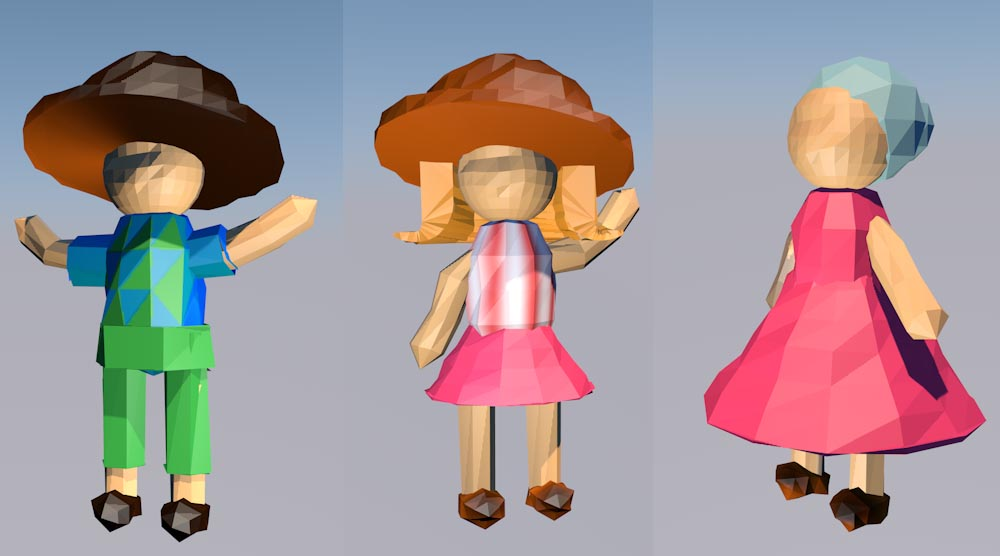
\includegraphics[width=0.9\textwidth]{images/Charaktere}
	\caption{Charaktermodelle}
	\label{fig:Frau1}
\end{figure}

Es gibt verschiedene Charaktere im Spiel:

\begin{itemize}
\item Wissenschaftler: Ist der Mentor des Spielers. Er ist aber gleichzeitig auch ein passiver Gegenspieler, da er der Verursacher des Weltenchaos ist. Er integriert den Spieler in seine eigene Welt und schickt ihn auf eine Heldenreise.
\item Spieler: Er ist der Protagonist und sieht die Welt mit seinen eigenen Augen. Er ist der Held des Spiels und hat die Möglichkeit die Welt des Wissenschaftlers zu retten.
\item Frau 1: Sie ist der erste NPC, mit dem der Spieler agiert. Sie trägt einen großen Hut und pinke Kleidung. Sie lebt schon seit ihrer Kindheit im Dorf und versteht sich mit allen sehr gut. Fremden gegenüber ist sie sehr offen und begrüßt den Spiele herzlich im Dorf. Animationen: Idle, Wave, Panic
\item Frau 2: Sie ist eine ältere Dame, die im Dorf lebt und dem Spieler das Gefühl gibt, nicht ganz alleine in der Welt zu sein. Gerne schaut sie aus ihrem kleinen Fenster und genießt das Leben im Dorf. Sie hat bereits graue Haare und trägt ein auffälliges pinkes Kleid. Sobald die Lichtmaschine wieder repariert ist, verlässt sie sofort ihr Haus. Animationen: Idle
\item Mann 1: Er ist der zweite NPC mit dem der Spieler interagiert. Durch den Vulkanausbruch steht sein Haus in Flammen und muss dringend gelöscht werden. Voller Panik wartet er auf Hilfe. Er trägt den dorftypischen Hut, ein blaues Oberteil und eine grüne Hose. Animationen: Idle, Wave, Panic
\item Mann 4: Er lebt mit seiner Familie in einem kleinen Haus am Rande des Dorfes. Seine Kinder spielen immer mit den Schafen. In letzter Zeit hat er Angst wenn die Kleinen draußen unterwegs sind. Jetzt, da das Licht wieder an ist jedoch nicht mehr. Auch er trägt das typische Dorfoutft. Animationen: Idle
\end{itemize}
\mysubsection{Sarah Häfele}{Dialoge}

Da der Spieler die ZEISS VR-ONE aufhat und damit die Welt stereoskopisch sieht, soll keine GUI das Blickfeld stören. Trotzdem muss die Story und das Gameplay vermittelt werden. Beides soll deshalb mit selbst eingesprochenen Dialogen dargestellt werden. Die Dialoge müssen natürlich klingen, um den Spieler nicht aus der Welt zu reißen und müssen trotzdem informativ genug sein, damit man weiß, was man tun muss. Der Rätsel- und Erkundungsdrang soll angeregt werden, weswegen die Dialoge nicht all zu viel verraten sollen.
Die Hauptperson, der verrückte Wissenschaftler (eingesprochen von Alexander Scheurer), übernimmt deshalb den Storypart - die Story wird so aus seiner Sicht leicht verwirrend erzählt, so dass der Spieler noch genug selbst herausfinden muss. Das Tutorial stellt die erste Aufgabe dar, bei der der Spieler Feedback durch unteranderem den Dialog mit einer Bewohnerin der Insel erhält (eingesprochen von Sarah Häfele). Die restlichen Aufgaben sollen daraufhin keine Dialoge mehr benötigen.
Zum Abschluss des Spiels bedankt sich der Wissenschaftler beim Spieler. 
\mysubsection{Sarah Häfele}{Audio-Setting}

Die Hintergrundmusik soll durch leichte Klavierklänge entspannend aber trotzdem interessant wirken. Hierbei wird aus Zeitmangel ein Stück aus Freesound.org eingespielt.

Umgebungs- und Tiersounds unterstreichen die Landschaften und die Dialoge helfen dem Spieler die Story und die Rätsel zu verstehen. Geräte wie die Gravitationsmaschine spielen Sound ab, um dem Spieler Feedback für Aktionen zu geben.

Ein Problem kann die Handy-Schale der VR-ONE darstellen. Wenn das mobile Endgerät nicht genau in die Schale passt, können unter Umständen die Audioeingänge verdeckt sein.

\textit{Anmerkung:} Die Umgebungsmusik und die Sounds sind die einzigen Assets, die nicht selbst gemacht wurden. Folgend aufgelistet finden sich die Links zu diesen Assets:

\begin{itemize}
\item Backgroundmusic Piano (Quelle: \url{https://www.freesound.org/people/ERH/sounds/163485/})
\item Sound Schafe (Quelle: \url{https://www.freesound.org/people/Gitanki/sounds/172712/})
\item Sound Robo Start (Quelle: \url{https://www.freesound.org/people/Ionicsmusic/sounds/196889/})
\item Sound Machine Start (Quelle: \url{https://www.freesound.org/people/qubodup/sounds/211993/})
\end{itemize}

%\input{Meta} --> wie alles mit dem cube zusammenhängt

\clearpage
\section{Levels und Welten}
\mysubsection{Sandra Beuck}{Allgemeine Struktur}

\begin{figure}[ht]%[htbp]
	\centering
		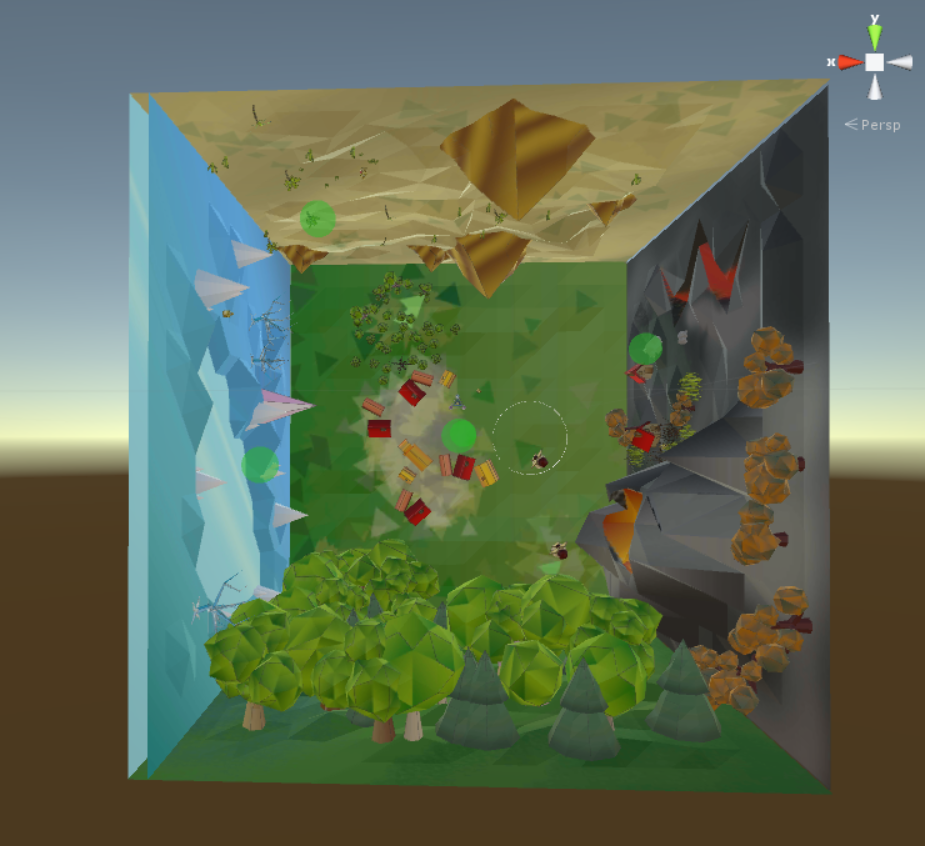
\includegraphics[width=1.0\textwidth]{images/worlds}
	\caption{Einblick in den Weltenwürfel aus Sicht der Gebirgswelt}
	\label{fig:Worlds}
\end{figure}

Das Spiel beziehungsweise der Würfel und seine Innenseiten bestehen aus insgesamt sechs Welten. Anstelle eines einzigen Themas für den gesamten Würfel, gibt es mehrere Themen innerhalb des Würfels geben, da unterschiedliche Themen mehr Potenzial für die Aufgabengenerierung bieten. Die Themen sollen nach ihrer Gegensätzlichkeit zueinander ausgewählt werden und dabei gleichzeitig in Bezug zu den vier Elementen des Seins stehen: Feuer, Wasser, Erde und Luft. Dadurch sind die Themen auch kontextuell miteinander verbunden. Die Welten, die sich im Würfel gegenüber liegen, bilden ein Paar, welchem ein gegensätzliches Thema zu Grunde liegen soll. Pro Paar ist der Spieler dazu aufgefordert, eine Aufgabe zu bewältigen, welche in Abhängigkeit zu den Paarwelten steht. Für die Aufgaben gibt es in jeder Welt eine aktive Zone, in welcher sich Triggerpunkte sowie Viewpoints befinden und mit denen der Nutzer interagieren soll.

Es werden folgende Themen für die Welten im Leveldesign umgesetzt: 

Gebirge und Dorf: Spiegeln die Elemente Luft und Erde wieder. 
Feuer und Eis: Stehen für die Elemente Feuer und Wasser.
Wüste und Wald: Repräsentieren die Elemente Feuer und Erde.
\mysubsection{Lydia Friedrich}{Papierprototyp}

\begin{figure}[!htbp]%[htbp]
	\centering
		\includegraphics[width=0.9\textwidth]{images/Papier}
	\caption{Papierprototyp}
	\label{fig:Papierprototyp}
\end{figure}

Um einen ersten Überblick über die Komplexität der Spielwelten zu erhalten, wird ein Papierprototyp im Maßstab 20:150 und einigen Objekten auf den Innenseiten des Würfels mit Pappe umgesetzt. Versuche ergeben, dass eine Größe von 200x200 m, besser für eine Weltenfläche geeignet ist, als eine Größe von nur 150x150 m. Deshalb sollte man im Vornherein, zeitgleich zur Erstellung des Papierprotoypen einen Tiefeneindrucktest durchführen, um die Vergleichbarkeit der optischen und tatsächlichen Wahrnehmung möglich zu machen. Es zeigt sich, dass der Abstand des Spielers im Würfel zu den Welten und dessen herausragenden Objekten, eine entscheidene Rolle für einen angenehmen stereoskopischen Wahrnehmungseindruck des Spielers spielt. Zudem kann durch eine Kombination des Papierprototypens und einem Tiefeneindrucktest die Größe der Objekte auf den Welten und deren Abstand zur Position des Spielers bestimmt werden. Die Größe der Objekte wird auf 1:5 der Weltenreite festgelegt.
\subsection{Welten}
\mysubsubsection{Lydia Friedrich}{Gebirgswelt}

Hallo

\mysubsubsection{Sandra Beuck}{Dorfwelt}

Hallo

\mysubsubsection{Sandra Beuck}{Waldwelt}

Hallo

\mysubsubsection{Lydia Friedrich}{Wüstenwelt}

Hallo

\mysubsubsection{Sandra Beuck}{Feuerwelt}

Hallo

\mysubsubsection{Lydia Friedrich}{Eiswelt}

Hallo
\mysubsection{Lydia Friedrich}{Aufgaben}

Das Leveldesign aller Welten befindet sich im Anhang (siehe Abbildungen \ref{Leveldesign})
\subsubsection{Gebirgswelt - Dorfwelt}
Der Spieler befindet sich im Inneren des Würfels in welchem es stockfinster ist. Grund hierfür ist die zusammengefaltete Welt, in welcher sich der Spieler befindet (die Sonne kommt nicht mehr hindurch). Zudem ist die Lichtmaschine defekt, welche alle Welten des Würfels mit Strom versorgt. Um die Lichtmaschine einzuschalten und das erste Remote Cube Teil zu erhalten, muss der Spieler in der Gebirgswelt den Triggerpunkt der Gravitationsmaschine aktivieren, damit die Kristalle, welche sich am Gebirge befinden, auf die Dorfwelt fallen. In der Dorfwelt muss ein Kristall nun in seine ursprüngliche Fassung hineingelegt werden. Um dies zu erreichen, muss der Spieler den Kristall eine gewisse Zeit fixieren um dessen Triggerpunkt auszulösen. Nachdem sich der Kristall wieder in seiner Fassung befindet, erwacht der Würfel zu neuem Leben und es wird hell. Der Spieler kann sich nun alle Welten des Würfels genauer ansehen. Doch bevor der Spieler die Aufgaben der anderen Welten lösen kann, muss er sich zunächst das Remote Cube Teil bei dem winkenden Einwohner des Dorfes zum Dank abholen, in dem er den Triggerpunkt des Einwohners aktiviert und gleichzeitig wird der \enquote{Dankesdialog} aktiviert.


Diese erste Welt dient als eine Art Tutorial für den Spieler und er erhält somit die Möglichkeit sich mit der Spielumgebung und der Spielsteuerung vertraut zu machen.

\subsubsection{Eiswelt - Feuerwelt}
Um in diesem Weltenpaar das ersehnte Remote Cube Teil zu bekommen, muss der Spieler zuerst auf der Feuerwelt den Vulkan ansehen, damit dessen Triggerpunkt ausgelöst wird und der Vulkan zu Spucken anfängt. Der Vulkan brodelt so stark, dass vereinzelt Lavabrocken in die umliegende Landschaft fliegen und dabei das Haus des einzigen Bewohners der Welt in Brand setzen. Um dem Einwohner zu helfen, indem der Spieler das Feuer löscht, muss der Triggerpunkt des Hauses ausgelöst werden, woraufhin der Spieler eine Fackel erhält. Mit dieser Fackel kann der Spieler in der Eiswelt den größten Eiszapfen zum Schmelzen bringen, indem er diesen lange fixiert und dadurch den Triggerpunkt des Eiszapfen auslöst. Im Anschluß muss der Spieler nur noch die Gravitationsmaschine durch einen Triggerpunkt aktivieren, damit das nun zu Wasser gewordene Eis auf das brennende Haus \enquote{hoch tropfen} kann und somit den Brand löscht. Der Spieler kann sich sein Remote Cube Teil beim Einwohner, mit Hilfe des Triggerpunktes, als Dank für seine Hilfe abholen.

\subsubsection{Wüstenwelt - Waldwelt}
Das Remote Cube Teil befindet sich in einem tiefen Loch in der Wüstenwelt. Eigentlich muss der Spieler nur das Gravitationsgerät einschalten, damit das Remote Cube Teil aus dem Loch heraus auf die Waldwelt fallen kann, jedoch ist das Gravitationsgerät unter Sand vergraben. Deshalb muss der Spieler zunächst in der Waldwelt eine Schaufel finden, welche an einen Holzstapel angelehnt ist. Durch Auslösen des Triggerspunktes, welcher sich auf der Schaufel befindet, kann der Spieler die Schaufel einsammeln. Mit Hilfe der Schaufel befreit der Spieler nun das Gravitationsgerät in der Wüstenwelt von dem Sand, dazu muss der Spieler auf den Sandhaufen über dem Gravitationsgerät den Triggerpunkt auslösen. Der Triggerpunkt auf dem Gravitationsgerät löst nun dessen Aktivität aus und das Remote Cube Teil fällt auf die Waldwelt und kann dort vom Spieler eingesammelt werden.
\mysubsection{Sandra Beuck}{Texturen}

Alle Modelle sind in Cinema4D Materialien (Farbe und Farbverläufe) ausgestattet. Die Wahl von flächigen Faben sowie zweifarbigen Verläufen dient zur Unterrstreichung der Low Poly Effekte. Desweiteren lässt sich somit die Tiefenstruktur optimal betonen.

Die fertigen Materialien werden in Cinema4D gebacken und als png´s exportiert. Die Texturen sind somit für Unity importfähig. Sofern es nötig ist werden die einzelnen gebackenen Texturen in Photshop nachbearbeitet und in Unity ersetzt.
%\mysubsection{Sandra Beuck}{Animationen}

Um dem Spiel mehr Leben einzuhauchen dient der Einsatz von Animationen. Alle Tiere und NPCs sind mit einer Kombination von klassischen Key-Frame- und Bone-Animation versehen. Einige Objekte haben mehrere Stati. So lässt sie sich per Skript ansteuern. Die NPCs befinden sich im \enquote{Idle}-Modus bis eine bestimmte Aktion des Spielers den \enquote{Action}-Modus auslöst.

Vorgehen:
\begin{itemize}
\item Erstellung eines Mashes aus mehreren Objekten
\item Einfärben / Texturieren
\item Zusammenfügen zu einem Objekt
\item Textur backen
\item Joints einfügen
\item Joints an das Objekt binden
\item Animation mit Hilfe der Joints / Key-Frame Animation
\item Export
\end{itemize}

Inverse Kinematik wirkt bei groben Polygonen sehr irritierend, deshalb genügt die einfache Animation um dem Spieler ein angenehmes Spielgefühl zu übermitteln. Die Probleme, die durch das Binden an ein Objekt entstehen, könnten durch Nachjustieren der Wichtung relativ einfach vermieden werden. In Anbetracht der kurzen Zeit haben jedoch viele Objekte sich überschneidende Polygone im Inneren. Dadurch wird die Wichtung komplizierter und teils kaum umsetzbar. Das Einbinden von Objekten in Unity mit Animation kann des Weiteren zu Störungen (fehlerhaftes Abspielen der Animation) führen, diese können mit erneuter Einbindung meist behoben werden. 


\clearpage
\section{Technik}
\mysubsection{Sarah Häfele}{Target Hardware}

InCubed ist für ein mobiles Engerät mit mindestens der Android Version 5, mit 3 GB Arbeitsspeicher, Octacore und Kamerafunktion entwickelt worden. Zudem wird die VR-/AR-Brille ZEISS-VR-ONE oder etwas ähnliches (wie z.B. das Google Cardboard) benötigt. Der für die Steuerung wichtige Markerwürfel wird durch die mitgelieferte Anleitung selber gebaut.
\mysubsection{Fabian Gärtner}{Development Hardware und Software}

Da die VR One von Zeiss mit ihrem Sichtfenster die Möglichkeit bietet, mittels der Kamera des Smartphones auch die Umgebung zu filmen und aus den in Kapitel X genannten Gründen, sollte neben der eigentlichen VR-Anwendung auch eine Art AR-Interaktion zum Einsatz kommen, um das Spiel interessanter zu gestalten. Zum einen geschieht das dadurch, wie in Kapitel X beschrieben, dass der Spieler zunächst die Realität über das Kamerabild sieht und schließlich über eine Art Wurmloch in das Spiel teleportiert wird, zum anderen durch die Bewegung in der virtuellen Welt mittels Bewegung eines Würfels in der echten Realität. Im Grunde wird hier also nicht die echte Realität, sondern die virtuelle Realität erweitert. Da es aber während des GameJams nicht möglich war, einen solchen Controller zur Steuerung in der Spielwelt mit Lagesensoren herzustellen, musste eine Möglichkeit gefunden werden, einzelne Seiten des Würfels lediglich mittels der zur Verfügung stehenden Smartphone-Kamera zu unterscheiden. In der Regel und auch bei inCubed geschieht eine solche Unterscheidung mittels verschiedener Marker. Solche Marker können in Form von QR-Codes, Bildern und anderen Strukturen gestaltet sein, erfordern dann allerdings eine Vielzahl an komplexen Algorithmen, um eine möglichst fehlerfreie Erkennung zu gewährleisten. In Anbetracht, dass für den GameJam aber lediglich eine begrenzte Zeit zur Verfügung stand, wurde in einem iterativen Prozess eine andere Art an Markern gesucht, die eine sehr einfache und effiziente und denoch genaue und zuverlässige Erkennung ermöglichen. So war zunächst die Idee, die sechs Seiten des Würfels unterschiedlich einzufärben und/oder mittels schwarzen Linien unterscheidbar zu machen. Da Farbe allein allerdings anfällig für schlechte Lichtverhältnisse ist, zeigte sich bei Tests mit verschiedenen Würfel-Prototypen aus Papier, dass die Verwendung von geometrischen Formen als Marker zu deutlich besseren Ergebnissen führt. Daher kommen nun beim fertigen Controller die sechs Formen Kreis, Dreieck, Viereck, Pentagon, Heptagon und Stern zum Einsatz, wobei auf den gegenüberliegenden Seiten des Würfels jeweils zwei möglichst unterschiedliche Formen zu finden sind. Die Erkennung dieser Formen ist beim Prototypen von inCubed vollständig implementiert und bereits ausreichend, um auch unter schlechten Lichtverhältnissen eine korrekte Erkennung zu ermöglichen. Für das fertige Spiel kann aber noch auf zwei Redundanzinformationen zurückgegriffen werden: Gegenüberliegende Formen haben, auch aus designtechnischen Gründen (siehe Kapitel X) dieselbe Farbe, sodass mittels zusätzlicher Farberkennung die erkannte Form verifiziert werden kann. Des Weiteren ist jede Würfelseite mit einer dicken schwarzen Linie umrandet, sodass der Suchprozess nach Markern auf die Erkennung eines Quadrates und eine anschließende Formerkennung innerhalb des Quadrates unterteilt werden kann. Außerdem ist so bestimmbar, welche der Würfelseiten die größte Fläche im Kamerabild einnimmt, falls der Nutzer den Würfel nicht optimal hält und dadurch mehrere Formen erkennbar wären.

Programmiertechnisch wird zur effizienten Markererkennung die kostenfreie Open-Source-Bibliothek OpenCV verwendet, die die Anwendung von Algorithmen und grundlegenden mathematischen Operationen auf Matrizen und Bilder ermöglicht. OpenCV stellt Wrapper für verschiedene Plattformen zur Verfügung, u.a. auch für Java und Android. Zwar könnte mit Hilfe der ebenfalls kostenfreien Bibliothek EmguCV OpenCV auch direkt aus C\# angesteuert werden, da die Zielplattform allerdings ein Android-System ist, müssten dann die OpenCV-Systemdateien (.so auf Android statt .dll auf Windows) ausgetauscht werden, was zu Problemen führen könnte. Daher wurde für inCubed eine andere Variante gewählt: Die Erkennung selbst wird in einer selbstgeschriebenen Java-/Android-Bibliothek unter Verwendung von OpenCV for Android vorgenommen. Diese Bibliothek wird anschließend als .jar-Datei exportiert und in Unity als sogenanntes Android-Plugin angesteuert. Bevor näher auf diese Plugin-Mechanik und die aufgetretenen Probleme eingegangen wird, soll zunächst das Plugin selbst genauer beschrieben werden. Nach Laden von OpenCV (der OpenCV-Manager muss als App auf dem Smartphone vorinstalliert sein, das Plugin kann diese App dann in der von Android bekannten OnResume-Funktion oder zu einem späteren Zeitpunkt starten und verwenden), wird die Verbindung zur Smartphone-Kamera hergestellt und mittels Eventsystem so verknüpft, dass das Plugin über jedes von der Kamera aufgenommene Kamerabild informiert wird. In einem extra Thread wird dieses Kamerabild dann in mehreren Schritten mittels diverser Algorithmen weiterverarbeitet und für die Markererkennung vorbereitet.

Welche Algorithmen für eine Markererkennung genau verwendet werden ist vom Einzelfall abhängig, in der Regel aber hat sich eine Mischung aus Kanten- und Konturerkennung sowie einer anschließenden Polygonannäherung als Vorgehensweise etabliert. Diese Algorithmen werden auch von OpenCV zur Verfügung stellt. Konkret wird bei inCubed eine Mischung aus Gaußschem Weichzeichner, adaptivem Threshold und dem sogenannten Canny-Edge-Detektor verwendet, um aus dem Kamerabild eindeutige Konturen zu extrahieren. Diese werden dann mittels Konturerkennungs-Algorithmus exakt beschrieben und durch Reduktion und Glättung der erkannten Punkte an einfache Polygone angenähert. Letztlich muss anschließend nur noch aufgrund der Eckpunktanzahl, der Fläche, der Form (konvex oder konkav) und der Winkel der Kanten zueinander entschieden werden, um welche Form es sich handelt. So ist bspw. der Stern die einzige konkave Form, der Kreis hat eine besonders hohe Zahl an Eckpunkten und Pentagon und Heptagon unterscheiden sich sowohl durch die Eckpunktanzahl als auch durch ihre Innenwinkel. Das Ergebnis dieser Erkennung und die Position der Bounding Box der Form sowie das Kamerabild wird anschließend an die Unity-Anwendung übergeben und von inCubed selbst weiterverarbeitet. Es zeigt sich hier, dass dieser Bildverarbeitungsprozess zwar relativ zeitaufwändig ist (letztlich aber immer noch effizienter als bei andernen Markerarten), aber sehr zuverlässig arbeitet und auch in dunkleren Räumen noch fehlerfrei die unterschiedlichen Formen erkennen kann. Durch die oben genannten Redundanzen könnte die Erkennung aber dennoch weiter verbessert werden. Für eine spätere Version des Spiels wäre es zudem denkbar Sensoren im Würfel zu platzieren, die mittels Bluetooth ihre Lage im Raum an das Smartphone senden. Dann könnte die Markererkennung zur Kalibrierung eingesetzt werden. Schon jetzt wird der Spieler zu Beginn des Spiels gebeten den Stern in die Kamera zu halten, sodass ein Kalibrierungsmodus jederzeit nachimplementiert werden kann.

Hier kommt nun das Pluginsystem von Unity zum Einsatz. Bereits im Plugin selbst kann durch Einbindung einer von Unity bereitgestellten classes.jar auf Unity-Funktionalität zurückgegriffen werden. So ist es bspw., nachdem der Nutzer seine Android-Activity von der UnityPlayerActivity abgeleitet hat, möglich, Nachrichten mittels SendMessage an beliebige GameObjects zu senden. Um ein solches Plugin dann in einer konkreten Unity-Anwendung einzusetzen, muss das Plugin als .jar-Datei exportiert und zusammen mit einer modifizierten AndroidManifest.xml in den Ordner Assets/Plugins/Android/ des jeweiligen Projektes gelegt werden. Unity bindet das Plugin dadurch automatisch in die Anwendung mit ein und ermöglicht es so, die im Plugin definierte Funktionalität aus C\# aus aufzurufen. Ein solcher Auruf kann wie in Listing X aussehen, wobei hier die im Plugin als öffentliche Methode definierte Methode "TestWert" aufgerufen wird und der Rückgabewert in einer Variable gespeichert wird.

CODE

Während dieses Pluginsystem durchaus Vorteile bietet und in inCubed auch zur Verwendung von Cardboard-Funktionalität zum Einsatz kommt, gibt es einige größere Nachteile, die die Entwicklung von inCubed zunächt beeinträchtigt haben. Die zur Verfügung stehenden Funktionalitäten sind zwar von Unity aus ausführlich dokumentiert (teilweise allerdings relativ unstrukturiert), in der Praxis waren aber dennoch viele schrittweise Tests erforderlich, um ein erstes lauffähiges Plugin zu implementieren. Gerade dadurch, dass ein selbstgeschriebenes Android-Manifest benötigt wird, dieses aber nicht ausführlich genug in der Doku erklärt wird, sind hier immer wieder Fehler aufgetreten. Des Weiteren gab es dadurch Probleme, dass auch das Cardboard-SDK als Android-Plugin ausgeliefert wird. Android selbst ist nicht dafür gemacht, dass mehrere Apps gleichzeitig aktiv sind. Es war daher zunächst nicht möglich sowohl VR- als auch AR-Funktionalität gleichzeitig einzusetzen. Dies führte zu Abstürzen von inCubed unter Ausgabe kryptischer Fehlermeldungen. Erst als dann das Cardboard-Plugin selbst durch die Funktionalität des selbstgeschriebenen Plugins erweitert und so letztlich nur noch ein Plugin benötigt wurde, war dieses Problem behoben. Aktuell ist nun hauptsächlich noch die Performance das größte Problem. Zwar liegt die Performance des Cardbord-Plugins als auch die Performance des selbstgeschrieben Markererkennungs-Plugins mit OpenCV auf dem verwendeten Samsung Galaxy S4 für sich genommen durchaus in einem vertretbarem Rahmen, arbeiten aber beide Plugins zusammen, zeigen sich größere Leistungseinbrüche. Dafür scheint es mehrere Gründe zu geben: zum einen ist das Galaxy S4 im Vergleich zu neueren Modellen nicht besonders leistungsstark, zum anderen verwendet Unity und OpenCV im Hintergrund ein Native Development Kit, um Funktionalität von Java nach C++ konvertieren zu können. Dies benötigt zusätzlich Leistung und Zeit, sodass es aktuell beim Intro und Outro von inCubed zu Performance-Einbrüchen kommt und das Kamerabild um etwa eine Sekunde verzöger angezeigt wird. Es ist davon auszugehen, dass sich auf einem Smartphone wie dem Samsung Galaxy S6, das auch mit der VR-One-Alternative GearVR ausgeliefert wird, solche Probleme deutlich weniger schwerwiegend auswirken sollten. Für einen Prototypen wie er während des GameJams entstanden ist, ist die schlechte Performance aber verzeihbar.


\clearpage
\section{Game Art}
\mysubsection{Lydia Friedrich}{Logo}

\begin{figure}[ht]%[htbp]
	\centering
		
\includegraphics[width=1.0\textwidth]{images/Logo}
	\caption{Logo inCubed}
	\label{fig:Logo}
\end{figure}

Das Logo ist eine Kombination aus einer Wort- und einer Bildmarke. Wobei die Bildmarke den Grundcharakter des Spiels widerspiegelt, sie besteht aus einem Quadrat an dessen oberen Seite sich ein umgedrehter Baum befindet. Die Farbe Blau symbolisiert die Freiheit, die dem Nutzer am Anfang des Spiels genommen wird.
\subsection{Models}

\mysubsubsection{Sandra Beuck}{Gravitationsmaschine}

\begin{figure}[!htbp]%[htbp]
	\centering
		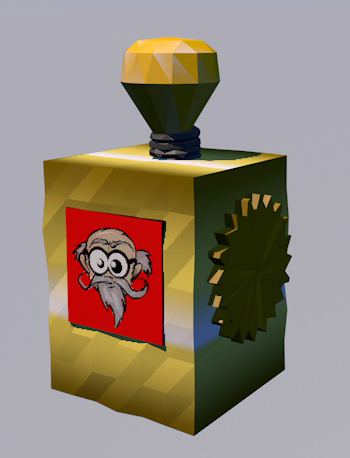
\includegraphics[width=0.8\textwidth]{images/gravinator}
	\caption{Gravitationsmaschine}
	\label{fig:gravinator}
\end{figure}

Die Gravitationsmaschine dient als Verbindungselement der Welten und ist in der Gebirgswelt prototypisch umgesetzt.

Sie ist eines der wichtigsten Elemente im Spiel, da sie in jeder Welt existent ist und somit ein Bezugspunkt für den Spieler darstellt. Aus diesem Grund ist die Gravitationsmaschine mit vielen Details, wie zum Beispiel einem Zahnrad, einem Bild des Wissenschaftlers und einer Kontrollleuchte versehen, und  erzeugt dadurch einen hohen Wiedererkennungswert. 

\mysubsubsection{Lydia Friedrich}{Remote Cube - Würfel}

\begin{figure}[!htbp]%[htbp]
	\centering
		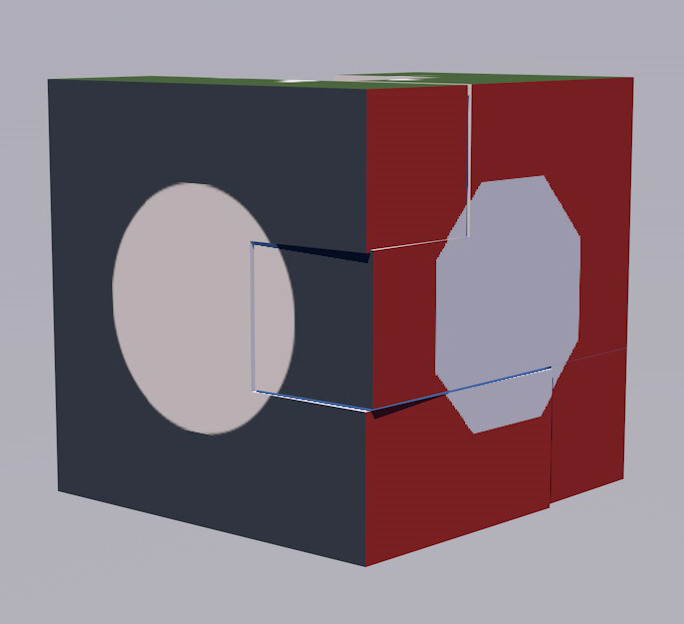
\includegraphics[width=0.8\textwidth]{images/RemoteCubeC4D}
	\caption{Virtueller Remote Cube}
	\label{fig:RemoteCube}
\end{figure}

Der Remote Cube ist die Verknüpfung des Würfels zur Außenwelt, denn nur mit ihm kann der Spieler das Spiel beenden und wieder in die reale Welt zurückkehren. Bevor dieses Ziel jedoch erreicht wird, müssen zunächst alle drei Teile des Remote Cubes erfolgreich vom Spieler eingesammelt werden (da der Remot Cube zu Beginn des Spiels zerbricht). Somit ist der Reomte Cube ebenfalls ein sehr wichtiges Spielelement da er das Symbol für den erfolgreichen Abschluß des Spiels darstellt.

Er ähnelt optisch dem Markerwürfel den der Spieler während des Spielens in den Händen hält und schafft so einen Bezug zwischen virtueller und realer Welt. Mit Hilfe von UV Mapping werden die Symbole des Markerwürfels auf den Remot Cube übertragen.

\clearpage
\section{Management}
%\mysubsection{Alexander Scheurer und Sarah Häfele}{Vorgehen}

\begin{figure}[!htbp]
	\centering
		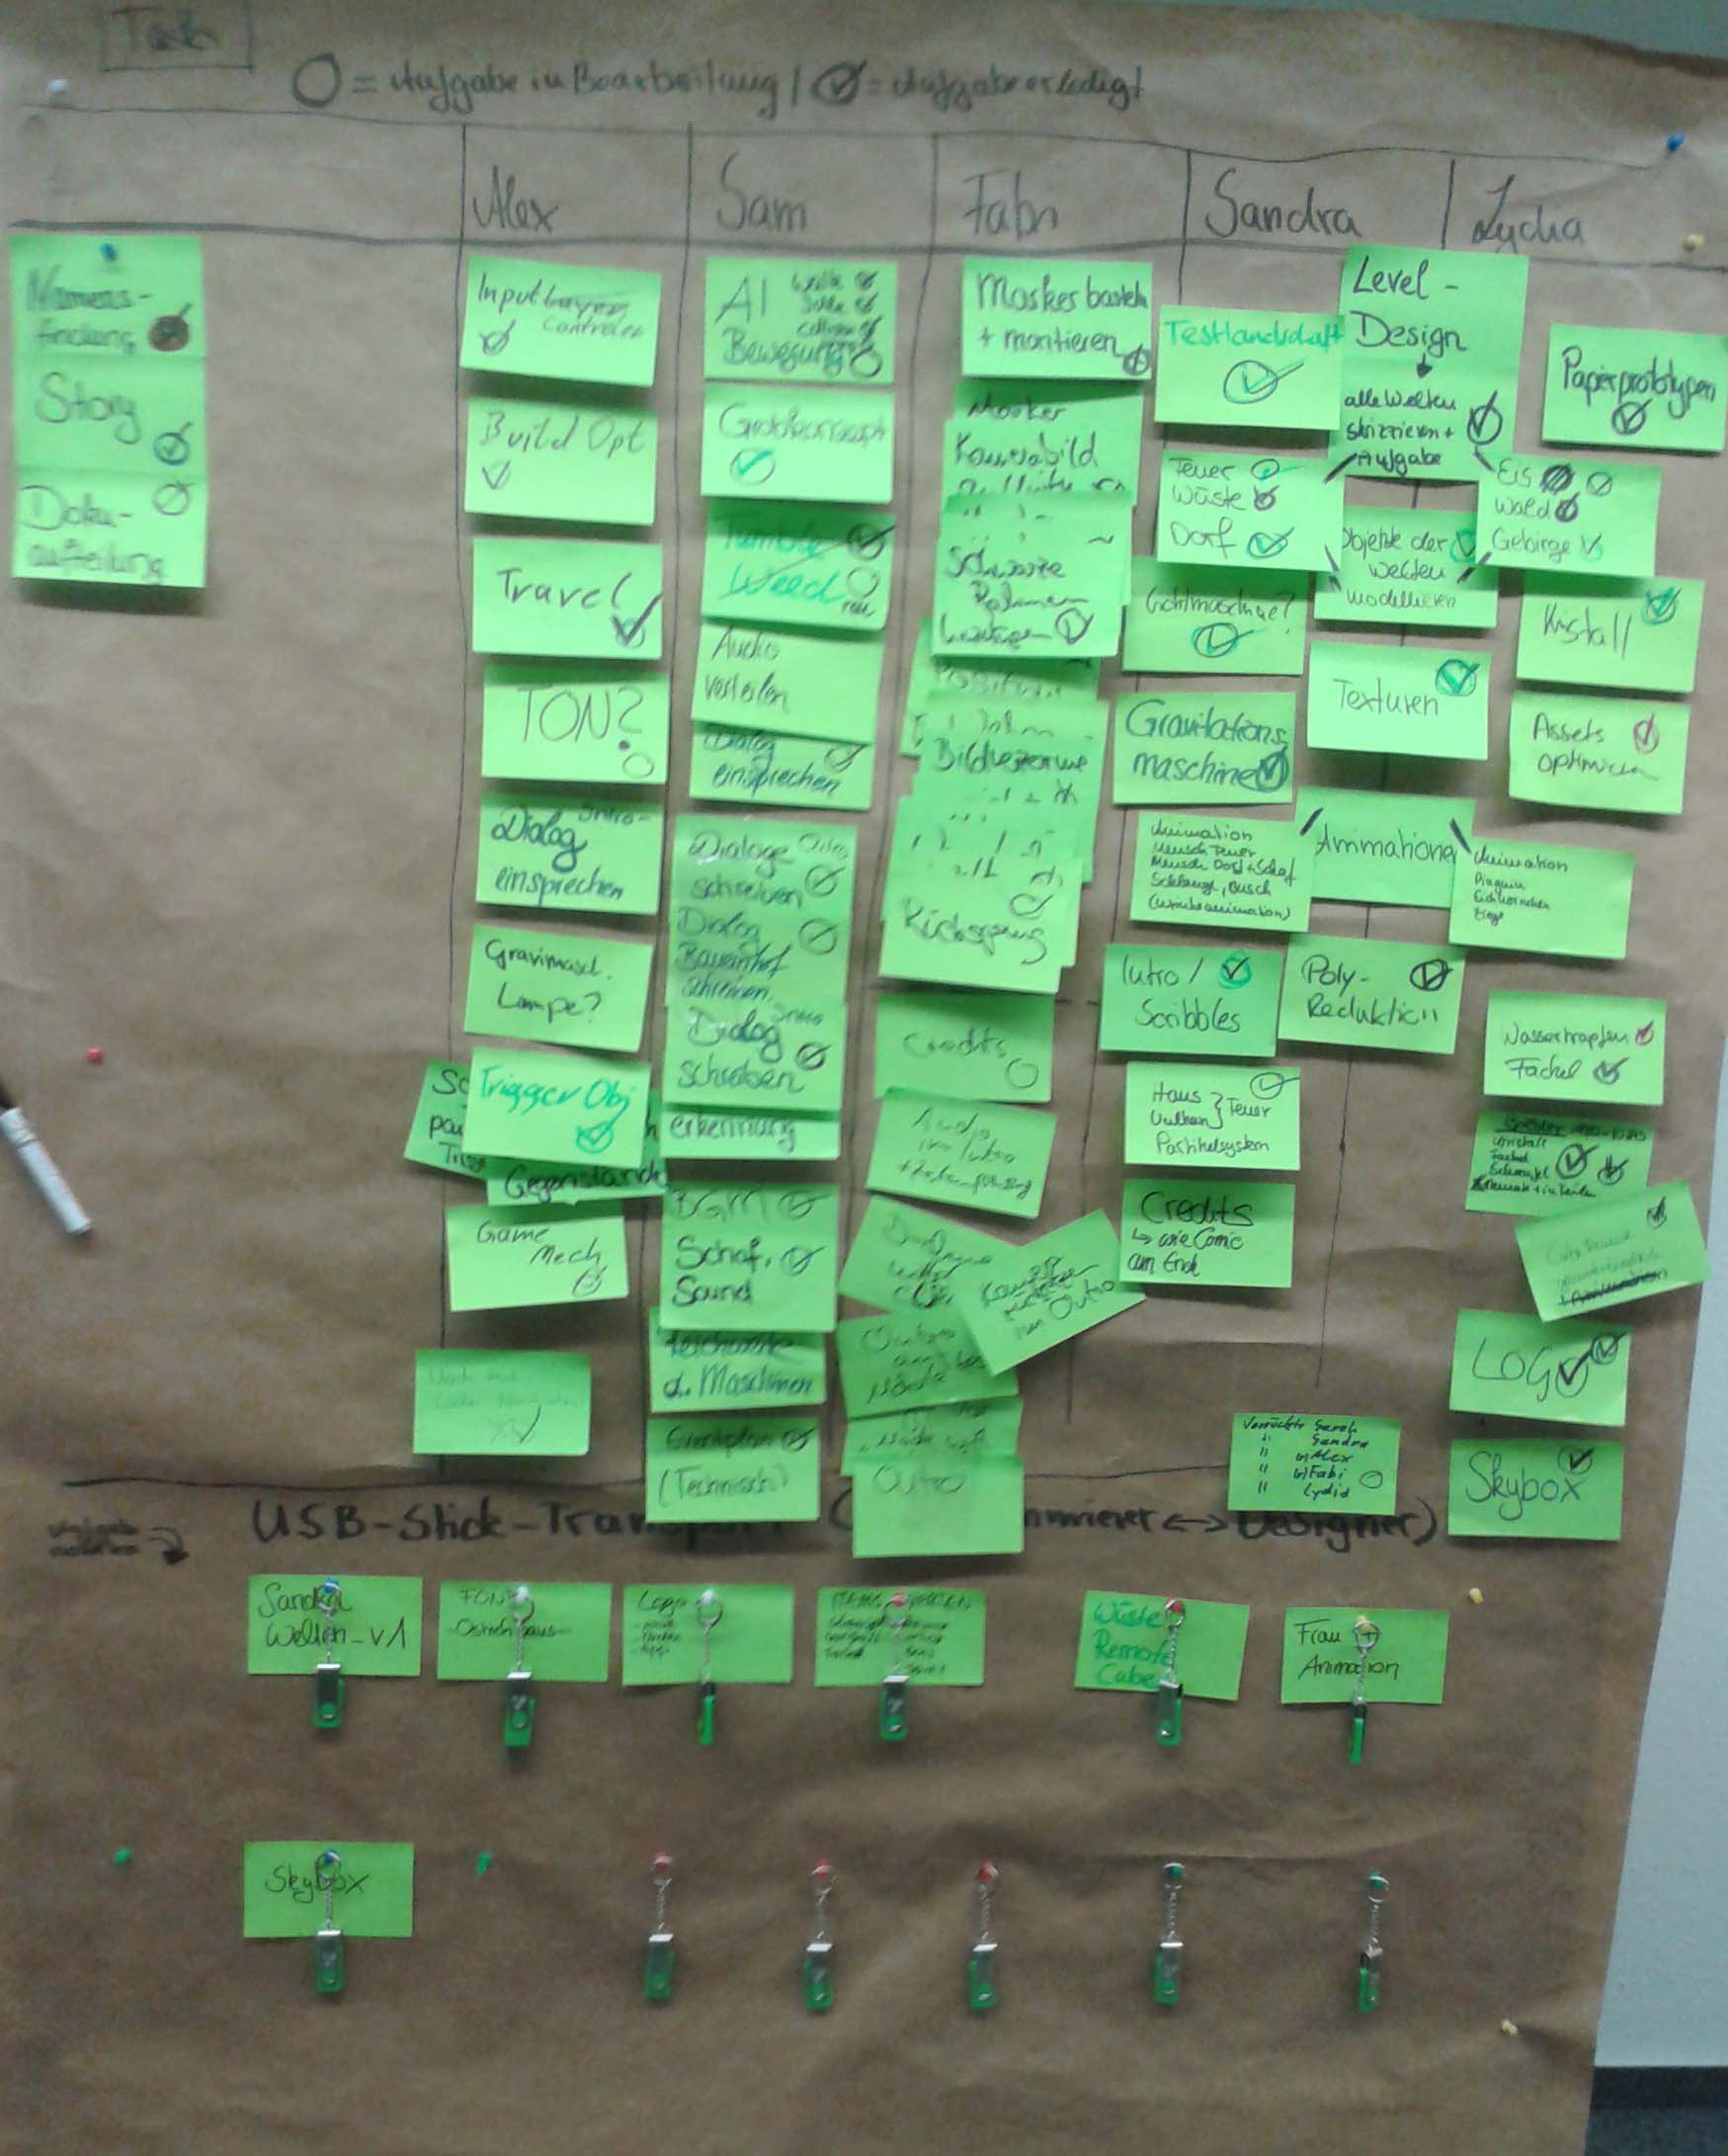
\includegraphics[width=1.0\textwidth]{images/Tasks}
	\caption{Taskboard}
	\label{fig:Tasks}
\end{figure}

Allgemeine Spieldesign-Entscheidungen wurden auf Whiteboards und Stehwänden erörtert und festgehalten. Daraus wurden Tasks gebildet, die auf einem Taskboard (siehe Abbildung \ref{fig:Tasks}) den einzelnen Teammitgliedern zugeordnet wurden. Angefangene und fertige Tasks wurden speziell markiert.

In tägliche kurzen Besprechungen am Morgen wurde festgelegt, welche Tasks bis zum Ende des Tages zu erfüllen sind (siehe Tabelle \ref{tab:Vorgehensweise}).

Einzelne Tasks wurden in Prototypen festgehalten und in eigenen Unity Szenen getestet. Das Projekt wurde durch Github versioniert. Notizen und das Designdokument wurde auf Google Drive geschrieben und in Latex zusammengefügt.

\begin{table}[!htbp]
\begin{center}
\begin{tabular}[hc]{l|l}
\hline
Mo & fertiges, grobes Konzept\\
& Welten und Aufgaben festlegen\\
& Markerprogrammierung\\
\hline
Di & Prototyp Papier\\
& Modellieren, Welten bauen\\
& Dialoge schreiben\\
& Grobkonzept\\
& 3D Tests der Welt\\
& Gamestates\\
\hline
Mi & Animationen\\
& Intro/Outro\\
& Gamestates und Trigger\\
& Dialoge einsprechen\\
& Sound\\
\hline
Do & Events finalisieren\\
& Outro mit Credits\\
& Doku beenden\\
\hline
Fr & Präsentation\\
\end{tabular}
\caption{Vorgehensweise}
\label{tab:Vorgehensweise}
\end{center}
\end{table}
%\input{Source Control}
%\input{Zeitplan, Sequenzdiagramm}
\mysubsection{Alexander Scheurer}{Zuständigkeiten}

Keine Entscheidung wurde alleine getroffen. Es war immer das gesamte Team beteiligt, sodass die hier angegebene Aufgabeneinteilung nur grob aufzufassen sind, da eigentlich jedes Teammitglied bei allen Punkten irgendwie mitgearbeitet hat.

\begin{table}[!htbp] %[hc]
\begin{center}
\begin{tabular}[hc]{l|l}
\hline
Sandra Beuck & Scribble Welten und Aufgaben\\
& Leveldesign: Wüste, Feuer, Dorf\\
& Comic - Intro und Outro\\
& Testlandschaft\\
& Animationen: Frau, Schlange, Windmühlen\\
\hline
Lydia Friedrich & Scribble Welten und Aufgaben\\
& Papierprototyp\\
& Leveldesign: Wald, Eis, Gebirge\\
& Model Remote Cube\\
& Item Karten\\
& Animationen:\\
& Charakter:\\
& Skybox\\
\hline
Fabian Gärtner & Markerbau und -programmierung\\
& Zusammenführung Android Plugin und Unity\\
& Programmierung von Intro und Outro\\
\hline
Sarah Häfele & Creature AI\\
& Verwaltung Design Doku\\
& Dialog Intro, Tutorial, Outro\\
& Sprecher Dialog Tutorial\\
& Storyboard Events (Eventplan)\\
& Eventsystem Unterstützung\\
& Sound Auswahl\\
\hline
Alexander Scheurer & Stresstest 3D\\
& Weltaufbau\\
& Gamemechanik Programmierung und Prototypen\\
& Eventsystem\\
& Sprecher Dialog Intro und Outro\\
& Controller Input\\
\end{tabular}
\caption{Zustaendigkeiten - Übersicht}
\label{tab:aufgaben}
\end{center}
\end{table}% --> tabelle

\clearpage
\section{Problemanalyse und Ausblick}

\clearpage
\section{Anhang}
\mysubsection{Sarah Häfele}{Dialoge}
\mysubsubsection{Sprecher: Alexander Scheurer}{Intro}

Du hältst etwas sehr wertvolles in den Händen: unsere Hoffnung. 
Man könnte meinen ich hätte alles unter Kontrolle… aber ich muss zugeben, ich habe mich verschätzt. 
Ich hatte etwas so wundervolles entdeckt. Dieser Ort ist nichts anderes als ein Würfel! Ein Würfel in Mitten von Meer! Aber niemand wollte mir glauben. Sie haben mich ausgelacht. Also wollte ich es ihnen zeigen. Beweisen, dass ich recht habe.
Und es hat viel zu gut funktioniert. Als ich meinen Fehler bemerkte, konnte ich nur noch diesen Hilferuf aussenden. 
Hier bist du also nun, ich bin genial, oder? Mir ist irgendwie die Fernbedienung verloren gegangen. Der Wind war zu stark. So ist das nunmal, wenn sich eine Insel zusammen klappt. Aber sie ist ein Würfel!
Jetzt ist es hier Dunkel, natürlich! Und ohne Fernbedienung kann die Insel nicht wieder aufgeklappt werden. 
Nun ist es so, ich bin etwas alt. Meine Füße machen das nicht mehr mit. Du kannst aber meine Gravitationsmaschinen verwenden, du wirst sie schon finden. Ist bisschen dunkel hier. Wir brauchen diese Fernbedienung! Viel Glück.

\mysubsubsection{Sprecher: Sarah Häfele}{Tutorial}

Huch, wer bist du denn? Hast du das Licht wieder angeschalten? Danke! Im Dunkeln konnte ich meine Finger nicht zählen, dabei war ich damit noch gar nicht fertig. Ich dachte schon: jetzt ist es soweit, ich werd verrückt. 
Das Ding hier hat mich dann aber überzeugt, dass ich’s wohl doch noch nicht bin. Ich hab mir ordentlich den Zeh daran gestoßen. 
Sieht so aus, als würde da was fehlen. Vielleicht findest du den Rest davon. Wenn du mich jetzt bitte entschuldigen würdest… ich hab da noch was wichtiges zu tun.

\mysubsubsection{Sprecher: Alexander Scheurer}{Outro}

Hast du das gesehen? Jetzt müssen sie mir glauben. Das war doch mal eine nette Abwechslung. Danke. Vielleicht können wir das jetzt jährlich machen…
Ach, du kannst jetzt gehen. 
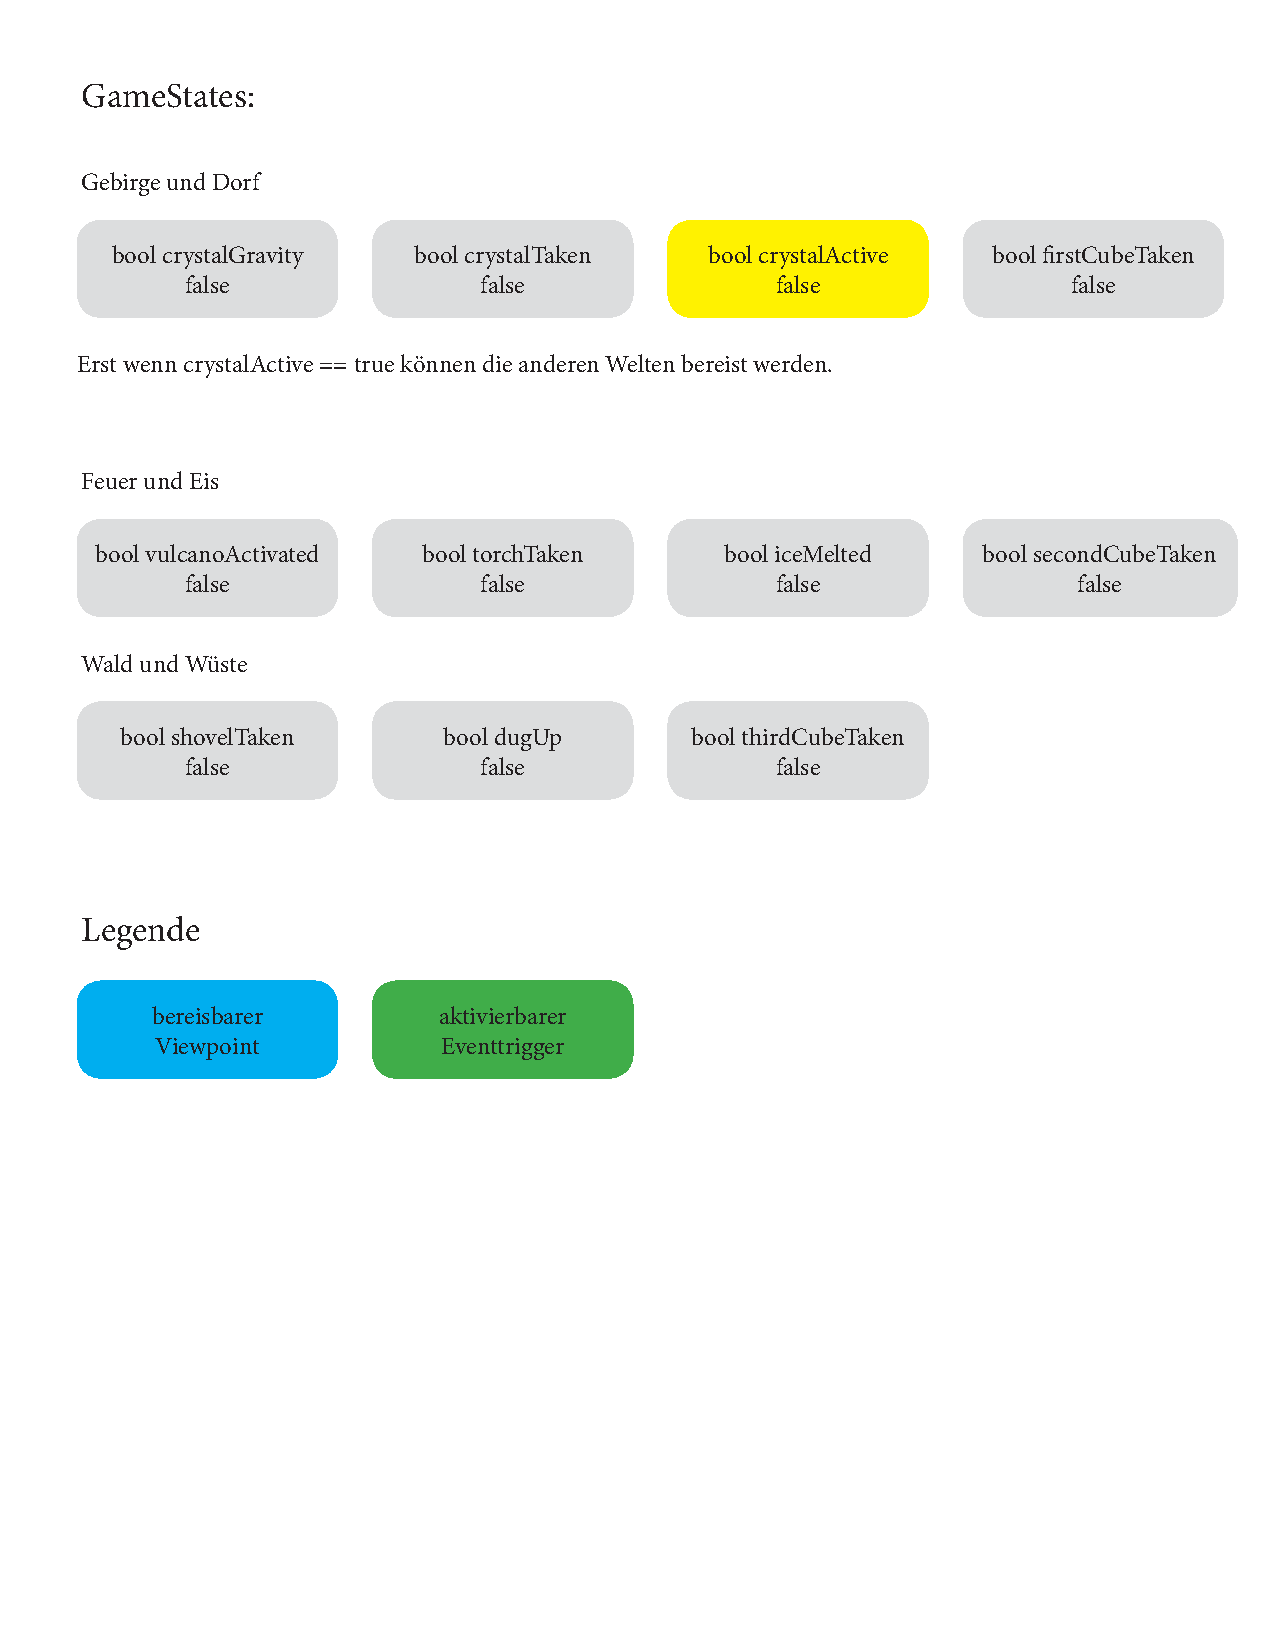
\includepdf[pages={1-8}]{appendix/statemachine.pdf}
%\input{Scribbles} etc.

\clearpage
\nocite{*}
\bibliographystyle{alphadin}
%\bibliography{bibliography}
\end{document}